\begin{frame}
	\frametitle{Pedosphäre - Böden}

	\begin{figure}
		\centering
		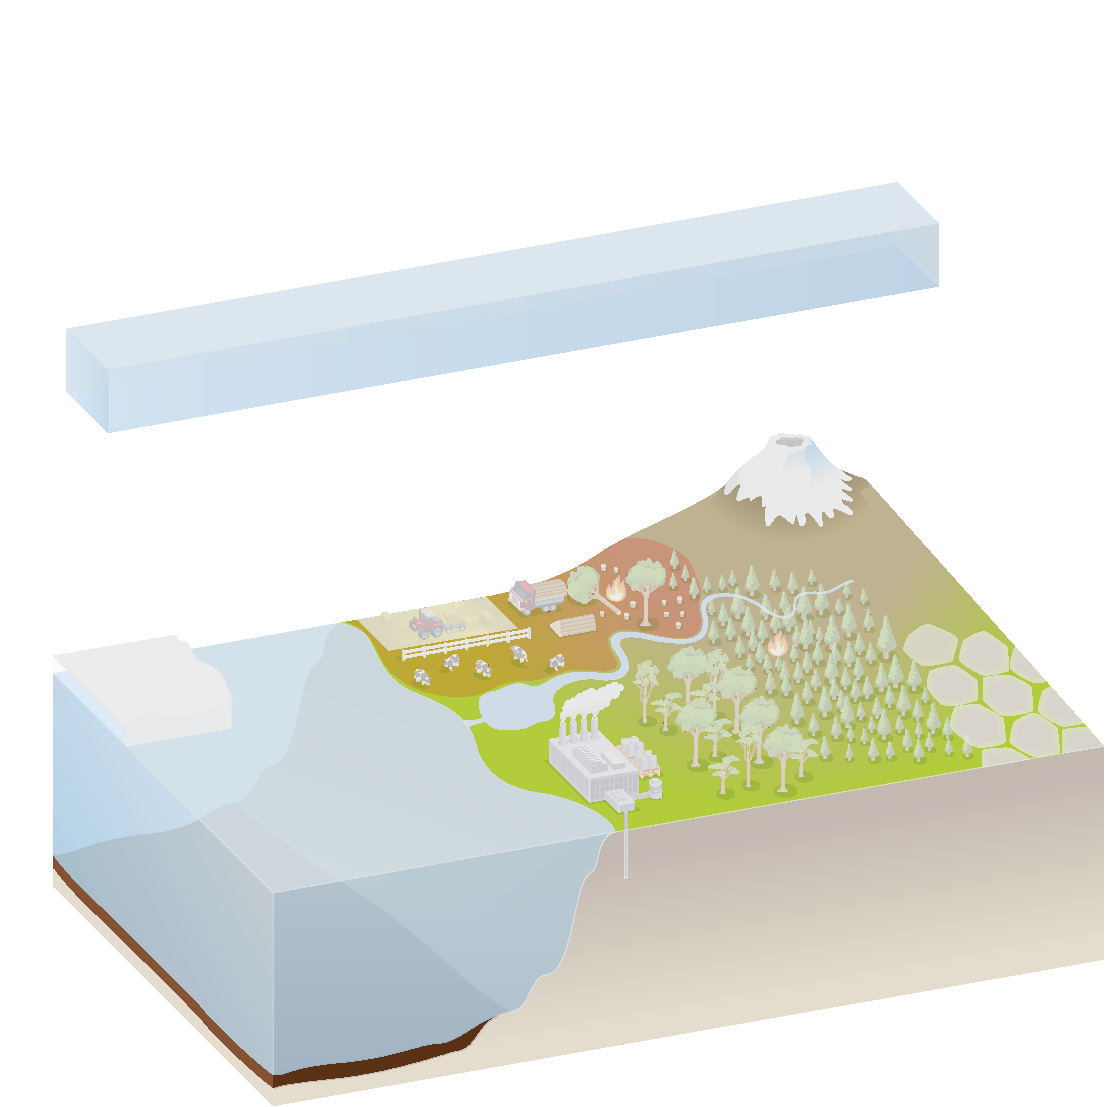
\includegraphics[trim={1cm 0cm 0cm 3cm}, clip, width=0.55\linewidth]{%
        bilder/climate_components/global_climate_components_pedosphere.pdf}
		\caption{Die Pedosphäre bezeichnet ist der Bereich der Erdoberfläche in dem sich Lithosphäre, Hydrosphäre, Atmosphäre und Biosphäre überschneiden.}
	\end{figure}

	\note{
		\begin{itemize}
			\item[] Pedosphäre bezeichnet den von Böden eingenommenen Bereich der Erdoberfläche, in dem sich die Lithosphäre, die Hydrosphäre, die Atmosphäre und die Biosphäre überschneiden.
			\item[] Ist Gestein atmosphärischen Einflüssen ausgesetzt (Niederschlag, Temperaturschwankungen usw.), verwittert es. Das verwitterte Gestein, gemischt mit zersetzter organischer Pflanzensubstanz, wird als Boden bezeichnet (Bodenbildung).
			\item[] Böden enthalten Wasser und Luft
			\item[$\rightarrow$] Überschneidung der Lithosphäre mit Hydrosphäre und Atmosphäre
			\item[] Im Boden leben Organismen
			\item[$\rightarrow$] Überschneidung Biosphäre und Pedosphäre
			\item[] Die Dicke der Pedosphäre schwankt stark: In kaltem und/oder trockenem Klima und in Hochlagen ist die Pedosphäre eher dünn (im cm Bereich), in warmem und feuchtem Klima und in Senken eher mächtig (dm Bereich). In den feuchten Tropen bis zu \SI{50}{m} und mehr.
		\end{itemize}
		Als Nächstes: Interaktionen, dazu erst ein Exkurs
	}
\end{frame}
